%%% Title:    Missing Data Stats Camp Course: Univariate MI
%%% Author:   Kyle M. Lang
%%% Created:  2017-SEP-12
%%% Modified: 2018-OCT-18

\documentclass{beamer}\usepackage[]{graphicx}\usepackage[]{color}
%% maxwidth is the original width if it is less than linewidth
%% otherwise use linewidth (to make sure the graphics do not exceed the margin)
\makeatletter
\def\maxwidth{ %
  \ifdim\Gin@nat@width>\linewidth
    \linewidth
  \else
    \Gin@nat@width
  \fi
}
\makeatother

\definecolor{fgcolor}{rgb}{0, 0, 0}
\newcommand{\hlnum}[1]{\textcolor[rgb]{0.69,0.494,0}{#1}}%
\newcommand{\hlstr}[1]{\textcolor[rgb]{0.749,0.012,0.012}{#1}}%
\newcommand{\hlcom}[1]{\textcolor[rgb]{0.514,0.506,0.514}{\textit{#1}}}%
\newcommand{\hlopt}[1]{\textcolor[rgb]{0,0,0}{#1}}%
\newcommand{\hlstd}[1]{\textcolor[rgb]{0,0,0}{#1}}%
\newcommand{\hlkwa}[1]{\textcolor[rgb]{0,0,0}{\textbf{#1}}}%
\newcommand{\hlkwb}[1]{\textcolor[rgb]{0,0.341,0.682}{#1}}%
\newcommand{\hlkwc}[1]{\textcolor[rgb]{0,0,0}{\textbf{#1}}}%
\newcommand{\hlkwd}[1]{\textcolor[rgb]{0.004,0.004,0.506}{#1}}%
\let\hlipl\hlkwb

\usepackage{framed}
\makeatletter
\newenvironment{kframe}{%
 \def\at@end@of@kframe{}%
 \ifinner\ifhmode%
  \def\at@end@of@kframe{\end{minipage}}%
  \begin{minipage}{\columnwidth}%
 \fi\fi%
 \def\FrameCommand##1{\hskip\@totalleftmargin \hskip-\fboxsep
 \colorbox{shadecolor}{##1}\hskip-\fboxsep
     % There is no \\@totalrightmargin, so:
     \hskip-\linewidth \hskip-\@totalleftmargin \hskip\columnwidth}%
 \MakeFramed {\advance\hsize-\width
   \@totalleftmargin\z@ \linewidth\hsize
   \@setminipage}}%
 {\par\unskip\endMakeFramed%
 \at@end@of@kframe}
\makeatother

\definecolor{shadecolor}{rgb}{.97, .97, .97}
\definecolor{messagecolor}{rgb}{0, 0, 0}
\definecolor{warningcolor}{rgb}{1, 0, 1}
\definecolor{errorcolor}{rgb}{1, 0, 0}
\newenvironment{knitrout}{}{} % an empty environment to be redefined in TeX

\usepackage{alltt}
\usetheme[%
  pageofpages          = of,
  bullet               = circle,
  titleline            = true,
  alternativetitlepage = true,
  titlepagelogo        = Logo3,
  watermark            = watermarkTiU,
  watermarkheight      = 100px,
  watermarkheightmult  = 4%
]{UVT}

\usepackage{graphicx}
\usepackage{booktabs}
\usepackage[natbibapa]{apacite}
\usepackage[libertine]{newtxmath}
\usepackage{fancybox}

\newcommand{\kfold}[0]{\emph{K}-fold cross-validation}

%% Ensure styles of `blocks' (used in Definitions, Theorems etc.) follows the
%% UVT-style theme:
\setbeamercolor{block title}{fg = darkblue, bg = white}
\setbeamercolor{block body}{use = block title, bg = block title.bg}

%% Ensure TableOfContents is in UVT-style theme:
\setbeamercolor{section in toc}{fg = darkblue}

\title{Univariate Multiple Imputation}
\subtitle{Stats Camp 2018: Missing Data Analysis}
\author{Kyle M. Lang}
\institute{Department of Methodology \& Statistics\\Tilburg University}
\date{19--21 October 2018}
\IfFileExists{upquote.sty}{\usepackage{upquote}}{}
\begin{document}

%------------------------------------------------------------------------------%



%------------------------------------------------------------------------------%

\begin{frame}[t,plain]

  \titlepage

\end{frame}

%------------------------------------------------------------------------------%

\begin{frame}{Outline}
  
  \begin{itemize}
  \item Build up the basis for MI from linear regression.
  \item Demonstrate each step with examples in R.
  \item Show how to manually implement a simple MI in R.
  \end{itemize}
  
\end{frame}

%------------------------------------------------------------------------------%

\begin{frame}{Brief Regression Refresher}
  
  Ordinary least squares (OLS) regression estimates the following model:
  \begin{align*}
    Y = \mathbf{X}\beta + \varepsilon
  \end{align*}
  By minimizing the residual sum of squared errors, we get the following 
  estimated regression coefficients:
  \begin{align*}
     \hat{\beta} = \left(\mathbf{X}^T \mathbf{X} \right)^{-1} \mathbf{X}^T Y
  \end{align*}
  We can predict the values of unobserved outcome data by applying the fitted 
  $\beta$s to new predictor data:
  \begin{align*}
    \hat{Y} = \mathbf{X}_{new}\hat{\beta}
  \end{align*}
  These predicted values are the basis for nearly all imputation methods.
  
\end{frame}

\watermarkoff %----------------------------------------------------------------%

\begin{frame}[fragile]{OLS Example}
    
\begin{knitrout}\scriptsize
\definecolor{shadecolor}{rgb}{0.878, 0.918, 0.933}\color{fgcolor}\begin{kframe}
\begin{alltt}
\hlcom{## Create some data:}
\hlstd{X}    \hlkwb{<-} \hlkwd{cbind}\hlstd{(}\hlnum{1}\hlstd{,} \hlkwd{rnorm}\hlstd{(}\hlnum{100}\hlstd{))}
\hlstd{beta} \hlkwb{<-} \hlkwd{matrix}\hlstd{(}\hlkwd{c}\hlstd{(}\hlnum{0.25}\hlstd{,} \hlnum{0.5}\hlstd{))}
\hlstd{y}    \hlkwb{<-} \hlstd{X} \hlopt \hlstd{beta} \hlopt{+} \hlkwd{rnorm}\hlstd{(}\hlnum{100}\hlstd{,} \hlnum{0.0}\hlstd{,} \hlnum{0.1}\hlstd{)}

\hlcom{## R's built-in solution:}
\hlstd{rFit} \hlkwb{<-} \hlkwd{lm}\hlstd{(y} \hlopt{~} \hlstd{X} \hlopt{-} \hlnum{1}\hlstd{)}
\hlkwd{coef}\hlstd{(rFit)} \hlcom{# R's fitted coefficients}
\end{alltt}
\begin{verbatim}
##        X1        X2 
## 0.2515459 0.4961789
\end{verbatim}
\begin{alltt}
\hlcom{## Least squares by hand:}
\hlstd{betaHat} \hlkwb{<-} \hlkwd{solve}\hlstd{(}\hlkwd{t}\hlstd{(X)} \hlopt \hlstd{X)} \hlopt \hlkwd{t}\hlstd{(X)} \hlopt \hlstd{y}
\hlkwd{t}\hlstd{(betaHat)} \hlcom{# Our hand-fitted coefficients}
\end{alltt}
\begin{verbatim}
##           [,1]      [,2]
## [1,] 0.2515459 0.4961789
\end{verbatim}
\end{kframe}
\end{knitrout}

\end{frame}

%------------------------------------------------------------------------------%

\begin{frame}[fragile]{OLS Example}

  \begin{columns}
    \begin{column}{0.5\textwidth}
      
\begin{knitrout}\footnotesize
\definecolor{shadecolor}{rgb}{0.878, 0.918, 0.933}\color{fgcolor}\begin{kframe}
\begin{alltt}
\hlcom{## What about prediction?}
\hlstd{X2}   \hlkwb{<-} \hlkwd{cbind}\hlstd{(}\hlnum{1}\hlstd{,} \hlkwd{rnorm}\hlstd{(}\hlnum{100}\hlstd{))}
\hlstd{yHat} \hlkwb{<-} \hlstd{X2} \hlopt \hlstd{betaHat}
\end{alltt}
\end{kframe}
\end{knitrout}

\end{column}
\begin{column}{0.5\textwidth}

\begin{knitrout}\footnotesize
\definecolor{shadecolor}{rgb}{0.878, 0.918, 0.933}\color{fgcolor}

{\centering 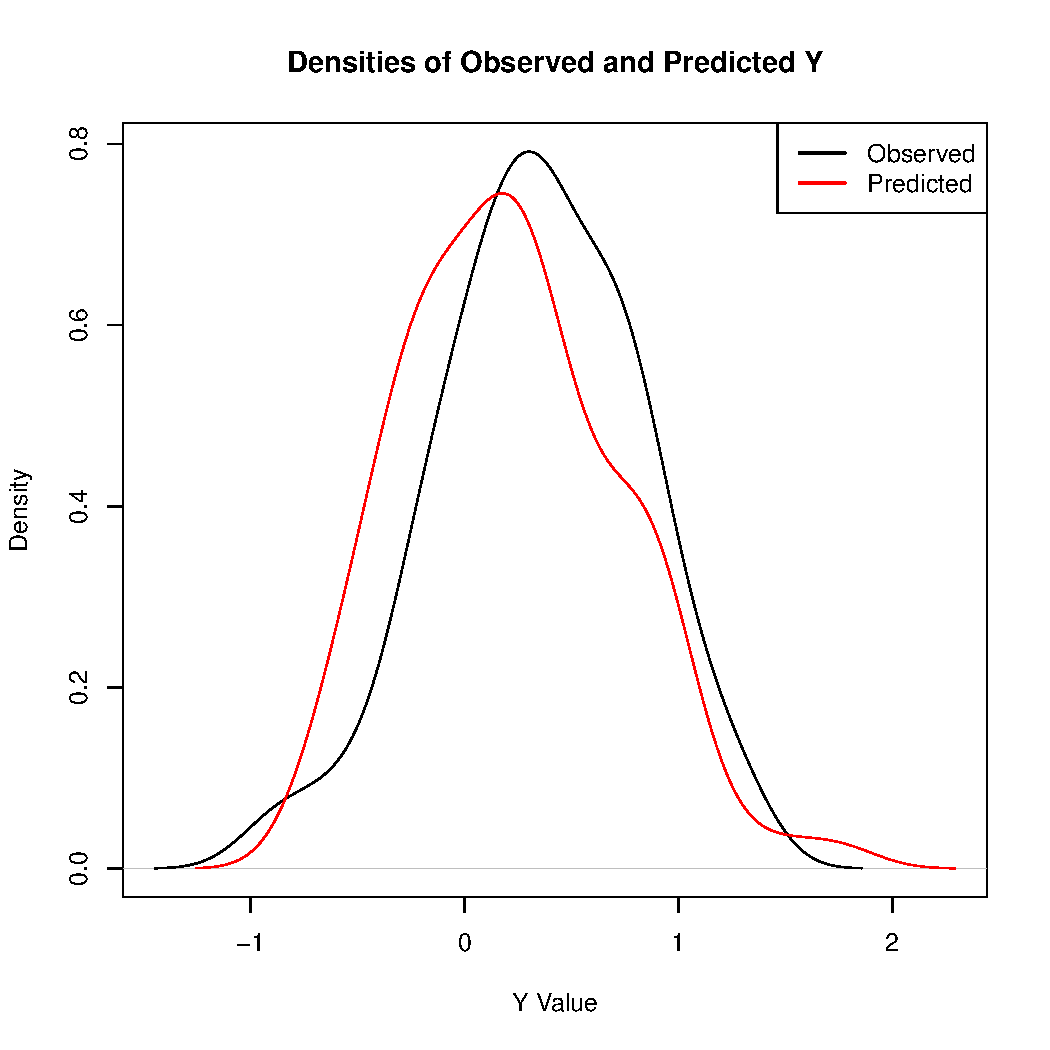
\includegraphics[width=\maxwidth]{figure/unnamed-chunk-3-1} 

}



\end{knitrout}

\end{column}
\end{columns}

\end{frame}

\watermarkon %-----------------------------------------------------------------%

\begin{frame}{Prediction}
  
  Train a model to predict BMI from diet-related and exercise-related features.
  \vb
  \begin{itemize}
  \item Plug-in new feature values corresponding to an experimental diet
    program to see the expected BMI for a hypothetical patient treated with the
    new program.  
  \end{itemize}
  \vb 
  Predict future gasoline prices based on geo-political events in
  oil-producing countries.  
  \vb
  \begin{itemize}
    \item If conflict escalates in the Middle East, adjust the appropriate
      features and project likely changes in gasoline prices.
  \end{itemize}
  
\end{frame}

%------------------------------------------------------------------------------%

\begin{frame}{Prediction Example}
  
  To fix ideas, let's consider the \emph{diabetes} data and the following model:
  \begin{align*}
    Y_{LDL} = \beta_0 + \beta_1 X_{BP} + \beta_2 X_{gluc} + \beta_3 X_{BMI} + 
    \varepsilon
  \end{align*}
  


Training this model on the first $N = 400$ patients' data produces the following
fitted model:
\begin{align*}
  Y_{LDL} = 22.135 + 0.089 X_{BP} + 0.498 X_{gluc} + 
  1.48 X_{BMI}
\end{align*}
\pause
Suppose a new patient presents with $BP = 121$, $gluc = 89$, and
$BMI = 30.6$. We can predict their $LDL$ score by:
\begin{align*}
  \hat{Y}_{LDL} &= 22.135 + 0.089 (121) + 0.498 
  (89) + 1.48 (30.6)\\
  &= 122.463
\end{align*}

\end{frame}

%------------------------------------------------------------------------------%

\begin{frame}{}
  
  \begin{center}
    \Huge{\textsc{Missing Data Imputation}}
  \end{center}
  
\end{frame}

%------------------------------------------------------------------------------%

\begin{frame}[shrink = 5]{Levels of Uncertainty Modeling}

  \citet{vanBuuren:2012} provides a very useful classification of different 
  imputation methods:
  \vb
  \begin{enumerate}
  \item Simple Prediction
    \begin{itemize}
    \item The missing data are naively filled with predicted values from some 
      regression equation.
    \item All uncertainty is ignored.
    \end{itemize}
    \vb
  \item Prediction + Noise
    \begin{itemize}
    \item A random residual error is added to each predicted value to create the 
      imputations.
    \item Only uncertainty in the predicted values is modeled.
    \item The imputation model itself is assumed to be correct and error-free.
    \end{itemize}
    \vb
  \item Prediction + Noise + Model Error
    \begin{itemize}
    \item Uncertainty in the imputation model itself is also modeled.
    \item Only way to get fully proper imputations in the sense of 
      \citet{rubin:1987}.
    \end{itemize}
  \end{enumerate}
  
\end{frame}

%------------------------------------------------------------------------------%

\begin{frame}[shrink = 5]{Do we really need to worry?}

  The arguments against single imputation can seem archaic and petty. Do we 
  really need to worry about this stuff?\\  
  \pause
  \vc
  \begin{itemize}
  \item YES!!! (At least if you care about inference)\\
  \end{itemize}
  \vb
  The following are results from a simple Monte Carlo simulation:
  
% latex table generated in R 3.5.1 by xtable 1.8-2 package
% Thu Oct 18 23:57:29 2018
\begin{table}[ht]
\centering
\scalebox{0.8}{
\begin{tabular}{rcccc}
  \toprule
 & Complete Data & Conditional Mean & Stochastic & MI \\ 
  \midrule
cor(X, Y) & 0.500 & 0.563 & 0.498 & 0.497 \\ 
  Type I Error & 0.052 & 0.138 & 0.120 & 0.054 \\ 
   \bottomrule
\end{tabular}
}
\caption{Mean Correlation Coefficients and Type I Error Rates} 
\end{table}


\pause
\vx{-12}
\begin{itemize}
\item Conditional mean substitution overestimates the correlation effect.
  \vc
\item Both single imputation methods inflate Type I error rates.
  \vc
\item MI provides unbiased point estimates and accurate Type I error rates.
\end{itemize}

\end{frame}

\watermarkoff %----------------------------------------------------------------%

\begin{frame}[fragile]{Simulate Some Toy Data}
  
\begin{knitrout}\scriptsize
\definecolor{shadecolor}{rgb}{0.878, 0.918, 0.933}\color{fgcolor}\begin{kframe}
\begin{alltt}
\hlstd{nObs} \hlkwb{<-} \hlnum{1000} \hlcom{# Sample Size}
\hlstd{pm}   \hlkwb{<-} \hlnum{0.3} \hlcom{# Proportion Missing}

\hlstd{sigma} \hlkwb{<-} \hlkwd{matrix}\hlstd{(}\hlkwd{c}\hlstd{(}\hlnum{1.0}\hlstd{,} \hlnum{0.5}\hlstd{,} \hlnum{0.0}\hlstd{,}
                  \hlnum{0.5}\hlstd{,} \hlnum{1.0}\hlstd{,} \hlnum{0.3}\hlstd{,}
                  \hlnum{0.0}\hlstd{,} \hlnum{0.3}\hlstd{,} \hlnum{1.0}\hlstd{),}
                \hlkwc{ncol} \hlstd{=} \hlnum{3}\hlstd{)}

\hlstd{simData} \hlkwb{<-} \hlkwd{as.data.frame}\hlstd{(}\hlkwd{rmvnorm}\hlstd{(nObs,} \hlkwd{c}\hlstd{(}\hlnum{0}\hlstd{,} \hlnum{0}\hlstd{,} \hlnum{0}\hlstd{), sigma))}
\hlkwd{colnames}\hlstd{(simData)} \hlkwb{<-} \hlkwd{c}\hlstd{(}\hlstr{"y"}\hlstd{,} \hlstr{"x"}\hlstd{,} \hlstr{"z"}\hlstd{)}

\hlcom{## Impose MAR Nonresponse:}
\hlstd{misData} \hlkwb{<-} \hlstd{simData}
\hlstd{rVec}    \hlkwb{<-} \hlkwd{pnorm}\hlstd{(misData}\hlopt{$}\hlstd{x,}
                 \hlkwc{mean} \hlstd{=} \hlkwd{mean}\hlstd{(misData}\hlopt{$}\hlstd{x),}
                 \hlkwc{sd}   \hlstd{=} \hlkwd{sd}\hlstd{(misData}\hlopt{$}\hlstd{x))} \hlopt{<} \hlstd{pm}
\hlstd{misData[rVec,} \hlstr{"y"}\hlstd{]} \hlkwb{<-} \hlnum{NA}

\hlcom{## Subset the data:}
\hlstd{yMis} \hlkwb{<-} \hlstd{misData[rVec, ]; yObs} \hlkwb{<-} \hlstd{misData[}\hlopt{!}\hlstd{rVec, ]}
\end{alltt}
\end{kframe}
\end{knitrout}

\end{frame}

%------------------------------------------------------------------------------%

\begin{frame}[fragile]{Look at the incomplete data.}

\begin{knitrout}\footnotesize
\definecolor{shadecolor}{rgb}{0.878, 0.918, 0.933}\color{fgcolor}\begin{kframe}
\begin{alltt}
\hlkwd{head}\hlstd{(misData,} \hlkwc{n} \hlstd{=} \hlnum{5}\hlstd{)}
\end{alltt}
\begin{verbatim}
##            y            x          z
## 1         NA -0.625895673 -1.2420694
## 2 -0.1448488 -0.001578954  0.4701091
## 3  1.2017766  1.069733846 -0.7550419
## 4  1.0424014 -0.192959605 -1.4458352
## 5  1.5970164 -0.249389277 -0.7206223
\end{verbatim}
\end{kframe}
\end{knitrout}

\end{frame}

%------------------------------------------------------------------------------%

\begin{frame}[fragile]{Expected Imputation Model Parameters}
    
\begin{knitrout}\footnotesize
\definecolor{shadecolor}{rgb}{0.878, 0.918, 0.933}\color{fgcolor}\begin{kframe}
\begin{alltt}
\hlcom{## Get the imputation model moments:}
\hlstd{lsFit} \hlkwb{<-} \hlkwd{lm}\hlstd{(y} \hlopt{~} \hlstd{x} \hlopt{+} \hlstd{z,} \hlkwc{data} \hlstd{= yObs)}

\hlstd{beta}  \hlkwb{<-} \hlkwd{coef}\hlstd{(lsFit)}
\hlstd{sigma} \hlkwb{<-} \hlkwd{summary}\hlstd{(lsFit)}\hlopt{$}\hlstd{sigma}

\hlstd{beta}
\end{alltt}
\begin{verbatim}
## (Intercept)           x           z 
##  0.03510861  0.55476584 -0.15346474
\end{verbatim}
\begin{alltt}
\hlstd{sigma}
\end{alltt}
\begin{verbatim}
## [1] 0.8595465
\end{verbatim}
\end{kframe}
\end{knitrout}

\end{frame}

%------------------------------------------------------------------------------%

\begin{frame}[fragile]{Conditional Mean Substitution}

\begin{knitrout}\footnotesize
\definecolor{shadecolor}{rgb}{0.878, 0.918, 0.933}\color{fgcolor}\begin{kframe}
\begin{alltt}
\hlcom{## Get deterministic imputations:}
\hlstd{imp1} \hlkwb{<-} \hlstd{beta[}\hlnum{1}\hlstd{]} \hlopt{+} \hlstd{beta[}\hlnum{2}\hlstd{]} \hlopt{*} \hlstd{yMis[ ,} \hlstr{"x"}\hlstd{]} \hlopt{+}
    \hlstd{beta[}\hlnum{3}\hlstd{]} \hlopt{*} \hlstd{yMis[ ,} \hlstr{"z"}\hlstd{]}

\hlcom{## Fill missing cells in Y:}
\hlstd{impData1}            \hlkwb{<-} \hlstd{misData}
\hlstd{impData1[rVec,} \hlstr{"y"}\hlstd{]} \hlkwb{<-} \hlstd{imp1}

\hlkwd{head}\hlstd{(impData1,} \hlkwc{n} \hlstd{=} \hlnum{5}\hlstd{)}
\end{alltt}
\begin{verbatim}
##            y            x          z
## 1 -0.1215031 -0.625895673 -1.2420694
## 2 -0.1448488 -0.001578954  0.4701091
## 3  1.2017766  1.069733846 -0.7550419
## 4  1.0424014 -0.192959605 -1.4458352
## 5  1.5970164 -0.249389277 -0.7206223
\end{verbatim}
\end{kframe}
\end{knitrout}

\end{frame}

%------------------------------------------------------------------------------%

\begin{frame}[fragile]{Stochastic Regression Imputation}
    
\begin{knitrout}\footnotesize
\definecolor{shadecolor}{rgb}{0.878, 0.918, 0.933}\color{fgcolor}\begin{kframe}
\begin{alltt}
\hlcom{## Get stochastic imputations:}
\hlstd{imp2} \hlkwb{<-} \hlstd{beta[}\hlnum{1}\hlstd{]} \hlopt{+} \hlstd{beta[}\hlnum{2}\hlstd{]} \hlopt{*} \hlstd{yMis[ ,} \hlstr{"x"}\hlstd{]} \hlopt{+}
    \hlstd{beta[}\hlnum{3}\hlstd{]} \hlopt{*} \hlstd{yMis[ ,} \hlstr{"z"}\hlstd{]} \hlopt{+} \hlkwd{rnorm}\hlstd{(}\hlkwd{nrow}\hlstd{(yMis),} \hlnum{0}\hlstd{, sigma)}

\hlcom{## Fill missing cells in Y:}
\hlstd{impData2}            \hlkwb{<-} \hlstd{misData}
\hlstd{impData2[rVec,} \hlstr{"y"}\hlstd{]} \hlkwb{<-} \hlstd{imp2}

\hlkwd{head}\hlstd{(impData2,} \hlkwc{n} \hlstd{=} \hlnum{5}\hlstd{)}
\end{alltt}
\begin{verbatim}
##            y            x          z
## 1  1.0827485 -0.625895673 -1.2420694
## 2 -0.1448488 -0.001578954  0.4701091
## 3  1.2017766  1.069733846 -0.7550419
## 4  1.0424014 -0.192959605 -1.4458352
## 5  1.5970164 -0.249389277 -0.7206223
\end{verbatim}
\end{kframe}
\end{knitrout}

\end{frame}

\watermarkon %-----------------------------------------------------------------%

\begin{frame}[fragile]{Flavors of MI}
  
  MI simply repeats a single regression imputation $M$ times.
  \begin{itemize}
  \item The specifics of the underlying regression imputation are important.
  \end{itemize}
  \vb
  \pause
  Simply repeating the stochastic regression imputation procedure described 
  above won't suffice.
  \begin{itemize}
  \item Still produces too many Type I errors
  \end {itemize}
  
% latex table generated in R 3.5.1 by xtable 1.8-2 package
% Thu Oct 18 23:57:29 2018
\begin{table}[ht]
\centering
\scalebox{0.8}{
\begin{tabular}{rccc}
  \toprule
 & Complete Data & PN-Type & PNE-Type \\ 
  \midrule
cor(X, Y) & 0.499 & 0.499 & 0.498 \\ 
  Type I Error & 0.040 & 0.066 & 0.046 \\ 
   \bottomrule
\end{tabular}
}
\caption{Mean Correlation Coefficients and Type I Error Rates} 
\end{table}


\vx{-16}
\begin{itemize}
\item Type I error rates for PN-Type MI are much better than they were for 
  single stochastic regression imputation, but they're still too high.
\end{itemize}

\end{frame}

%------------------------------------------------------------------------------%

\begin{frame}{Proper MI}
  
  The problems on the previous slide arise from using the same regression 
  coefficients to create each of the $M$ imputations.
  \begin{itemize}
  \item Implies that you're using the ``correct'' coefficients.
    \vb
  \item This assumption is plainly ridiculous.
    \begin{itemize}
    \item If we don't know some values of our outcome variable, how can we know 
      the ``correct'' coefficients to link the incomplete outcome to the 
      observed predictors?
    \end{itemize}
    \vb
    \pause
  \item Proper MI also models uncertainty in the regression coefficients used to 
    create the imputations.
    \begin{itemize}
    \item A different set of of coefficients is randomly sampled (using Bayesian 
      simulation) to create each of the $M$ imputations.
      \vc
    \item The tricky part about implemented MI is deriving the distributions 
      from which to sample these coefficients.
    \end{itemize}
  \end{itemize}
  
\end{frame}

%------------------------------------------------------------------------------%

\begin{frame}{Setting Up Proper MI}
  
  Our imputation model is simply a linear regression model:
  \begin{align*}
    Y = \mathbf{X} \beta + \varepsilon
  \end{align*}
  To fully account for model uncertainty, we need to randomly sample both 
  $\beta$ and $\text{var}(\varepsilon) = \sigma^2$.
  \begin{itemize}
  \item \textsc{Question:} Why do we only sample $\sigma^2$ and not 
    $\varepsilon$?
  \end{itemize}
  \pause
  \va
  For a simple imputation model with a normally distributed outcome and 
  uninformative priors, we need to specify two distributions:
  \begin{enumerate}
    \item The marginal posterior distribution of $\sigma^2$
    \item The conditional posterior distribution of $\beta$ 
  \end{enumerate}
  
\end{frame}

%------------------------------------------------------------------------------%

\begin{frame}{Marginal Distribution of $\sigma^2$}
 
  We first specify the marginal posterior distribution for the noise variance,
  $\sigma^2$.
  \vc
  \begin{itemize}
  \item This distribution does not depend on any other parameters.
  \end{itemize}
  \begin{align}
    \sigma^2 &\sim \text{Inv-}\chi^2 \left(N - P, MSE \right) \label{sigma2PosteriorEq}\\
    &\text{with } MSE = \frac{1}{N - P} \left( Y - \mathbf{X}\hat{\beta}_{ls} \right)^T \left( Y - \mathbf{X}\hat{\beta}_{ls} \right) \notag
  \end{align}
  \vx{-12}
  \begin{itemize}
  \item $\sigma^2$ follows a scaled inverse $\chi^2$ distribution.
  \end{itemize}

\end{frame}

%------------------------------------------------------------------------------%

\begin{frame}{Conditional Distribution of $\beta$}

  We then specify the conditional posterior distribution for $\beta$. 
  \vc
  \begin{itemize}
  \item This distribution is conditioned on a specific value of $\sigma^2$.
  \end{itemize}
  \begin{align}
    \beta \sim \text{MVN} \left( \hat{\beta}_{ls}, ~ \sigma^2 (\mathbf{X}^T \mathbf{X})^{-1} \right) \label{betaPosteriorEq}
  \end{align}
  \vx{-12}
  \begin{itemize}
  \item $\beta$ (conditionally) follows a multivariate normal distribution.
  \end{itemize}

\end{frame}

%------------------------------------------------------------------------------%

\begin{frame}{PPD of the Missing Data}
  
  Once we've sampled our imputation model parameters, we can construct the 
  posterior predictive distribution of the missing data.
  \vc
  \begin{itemize}
  \item This is the distribution from which we sample our imputed values.
    \vc
  \item In practice, we directly compute the imputations based on the simulated 
    imputation model parameters.
  \end{itemize}
  \begin{align}
    Y_{imp} &= \mathbf{X}_{mis}\tilde{\beta} + \tilde{\varepsilon} \label{impPosteriorEq}\\
    &\text{with } \varepsilon \sim \text{N} \left( 0, \widetilde{\sigma^2} \right) \notag
  \end{align}
  
\end{frame}

%------------------------------------------------------------------------------%

\begin{frame}{General Steps for Basic MI}
  
  With all of the elements in place, we can execute a basic MI by following 
  these steps:
  \vb
  \begin{enumerate}
  \item Find the least squares estimates of $\beta$, $\hat{\beta}_{ls}$, by 
    regressing the observed portion of $Y$ onto the the analogous rows of 
    $\mathbf{X}$.
    \vb
  \item Use $\hat{\beta}_{ls}$ to parameterize the posterior distribution of 
    $\sigma^2$, given by Equation \ref{sigma2PosteriorEq}, and draw $M$ samples 
    of $\sigma^2$ from this distribution.
    \vb
  \item For each of the $\sigma^2_m$, sample a corresponding value of $\beta$ 
    from Equation \ref{betaPosteriorEq}.
    \vb
  \item Plug the $M$ samples of $\beta$ and $\sigma^2$ into Equation 
    \ref{impPosteriorEq} to create the $M$ imputations.
  \end{enumerate}
  
\end{frame}

\watermarkoff %----------------------------------------------------------------%

\begin{frame}[fragile]{Manual MI Example}
      
  First, we need to sample from the marginal posterior distribution of
  $\sigma^2$.
  
\begin{knitrout}\footnotesize
\definecolor{shadecolor}{rgb}{0.878, 0.918, 0.933}\color{fgcolor}\begin{kframe}
\begin{alltt}
\hlcom{## Define iteration numbers:}
\hlstd{nImps} \hlkwb{<-} \hlnum{100}
\hlstd{nSams} \hlkwb{<-} \hlnum{5000}

\hlcom{## Get the expected betas:}
\hlstd{fit0}  \hlkwb{<-} \hlkwd{lm}\hlstd{(y} \hlopt{~} \hlstd{.,} \hlkwc{data} \hlstd{= yObs)}
\hlstd{beta0} \hlkwb{<-} \hlkwd{coef}\hlstd{(fit0)}

\hlcom{## Sample sigma:}
\hlstd{sigScale}  \hlkwb{<-} \hlstd{(}\hlnum{1} \hlopt{/} \hlstd{fit0}\hlopt{$}\hlstd{df)} \hlopt{*} \hlkwd{crossprod}\hlstd{(}\hlkwd{resid}\hlstd{(fit0))}
\hlstd{sigmaSams} \hlkwb{<-}
    \hlkwd{rinvchisq}\hlstd{(nSams,} \hlkwc{df} \hlstd{= fit0}\hlopt{$}\hlstd{df,} \hlkwc{scale} \hlstd{= sigScale)}
\end{alltt}
\end{kframe}
\end{knitrout}

\end{frame}

%------------------------------------------------------------------------------%

\begin{frame}[fragile]{Manual MI Example}
  
  Then we need to use those samples of $\sigma^2$ to parameterize the
  conditional posterior distribution of $\beta$ and sample from it.
  
\begin{knitrout}\footnotesize
\definecolor{shadecolor}{rgb}{0.878, 0.918, 0.933}\color{fgcolor}\begin{kframe}
\begin{alltt}
\hlcom{## Partition the predictor matrix:}
\hlstd{misX} \hlkwb{<-} \hlkwd{as.matrix}\hlstd{(}\hlkwd{cbind}\hlstd{(}\hlnum{1}\hlstd{, yMis[ ,} \hlkwd{c}\hlstd{(}\hlstr{"x"}\hlstd{,} \hlstr{"z"}\hlstd{)]))}
\hlstd{obsX} \hlkwb{<-} \hlkwd{as.matrix}\hlstd{(}\hlkwd{cbind}\hlstd{(}\hlnum{1}\hlstd{, yObs[ ,} \hlkwd{c}\hlstd{(}\hlstr{"x"}\hlstd{,} \hlstr{"z"}\hlstd{)]))}

\hlcom{## Sample beta:}
\hlstd{betaSams} \hlkwb{<-} \hlkwd{matrix}\hlstd{(}\hlnum{NA}\hlstd{, nSams,} \hlkwd{ncol}\hlstd{(obsX))}
\hlkwa{for}\hlstd{(i} \hlkwa{in} \hlnum{1} \hlopt{:} \hlstd{nSams) \{}
    \hlstd{betaVar}       \hlkwb{<-} \hlstd{sigmaSams[i]} \hlopt{*} \hlkwd{solve}\hlstd{(}\hlkwd{crossprod}\hlstd{(obsX))}
    \hlstd{betaSams[i, ]} \hlkwb{<-}
        \hlkwd{rmvnorm}\hlstd{(}\hlnum{1}\hlstd{,} \hlkwc{mean} \hlstd{= beta0,} \hlkwc{sigma} \hlstd{= betaVar)}
\hlstd{\}}
\end{alltt}
\end{kframe}
\end{knitrout}

\end{frame}

%------------------------------------------------------------------------------%

\begin{frame}[fragile]{Manual MI Example}
  
  Finally, we use the sampled imputation model moments to construct the missing 
  data's posterior predictive distribution:
  
\begin{knitrout}\footnotesize
\definecolor{shadecolor}{rgb}{0.878, 0.918, 0.933}\color{fgcolor}\begin{kframe}
\begin{alltt}
\hlstd{nMis}   \hlkwb{<-} \hlkwd{sum}\hlstd{(rVec)}
\hlstd{impMat} \hlkwb{<-} \hlkwd{matrix}\hlstd{(}\hlnum{NA}\hlstd{, nMis, nSams)}
\hlkwa{for}\hlstd{(i} \hlkwa{in} \hlnum{1} \hlopt{:} \hlstd{nSams) \{}
    \hlstd{impMat[ , i]} \hlkwb{<-} \hlstd{misX} \hlopt \hlkwd{matrix}\hlstd{(betaSams[i, ])} \hlopt{+}
        \hlkwd{rnorm}\hlstd{(nMis,} \hlnum{0}\hlstd{,} \hlkwd{sqrt}\hlstd{(sigmaSams[i]))}
\hlstd{\}}

\hlcom{## Fill the missing cells with the M imputations:}
\hlstd{impList} \hlkwb{<-} \hlkwd{list}\hlstd{()}
\hlstd{ind}     \hlkwb{<-} \hlkwd{sample}\hlstd{(}\hlnum{1} \hlopt{:} \hlstd{nSams)}
\hlkwa{for}\hlstd{(m} \hlkwa{in} \hlnum{1} \hlopt{:} \hlstd{nImps) \{}
    \hlstd{impList[[m]]}            \hlkwb{<-} \hlstd{misData}
    \hlstd{impList[[m]][rVec,} \hlstr{"y"}\hlstd{]} \hlkwb{<-} \hlstd{impMat[ , ind[m]]}
\hlstd{\}}
\end{alltt}
\end{kframe}
\end{knitrout}

\end{frame}

%------------------------------------------------------------------------------%

\begin{frame}{What do we get?}
    
\begin{knitrout}\footnotesize
\definecolor{shadecolor}{rgb}{0.878, 0.918, 0.933}\color{fgcolor}

{\centering 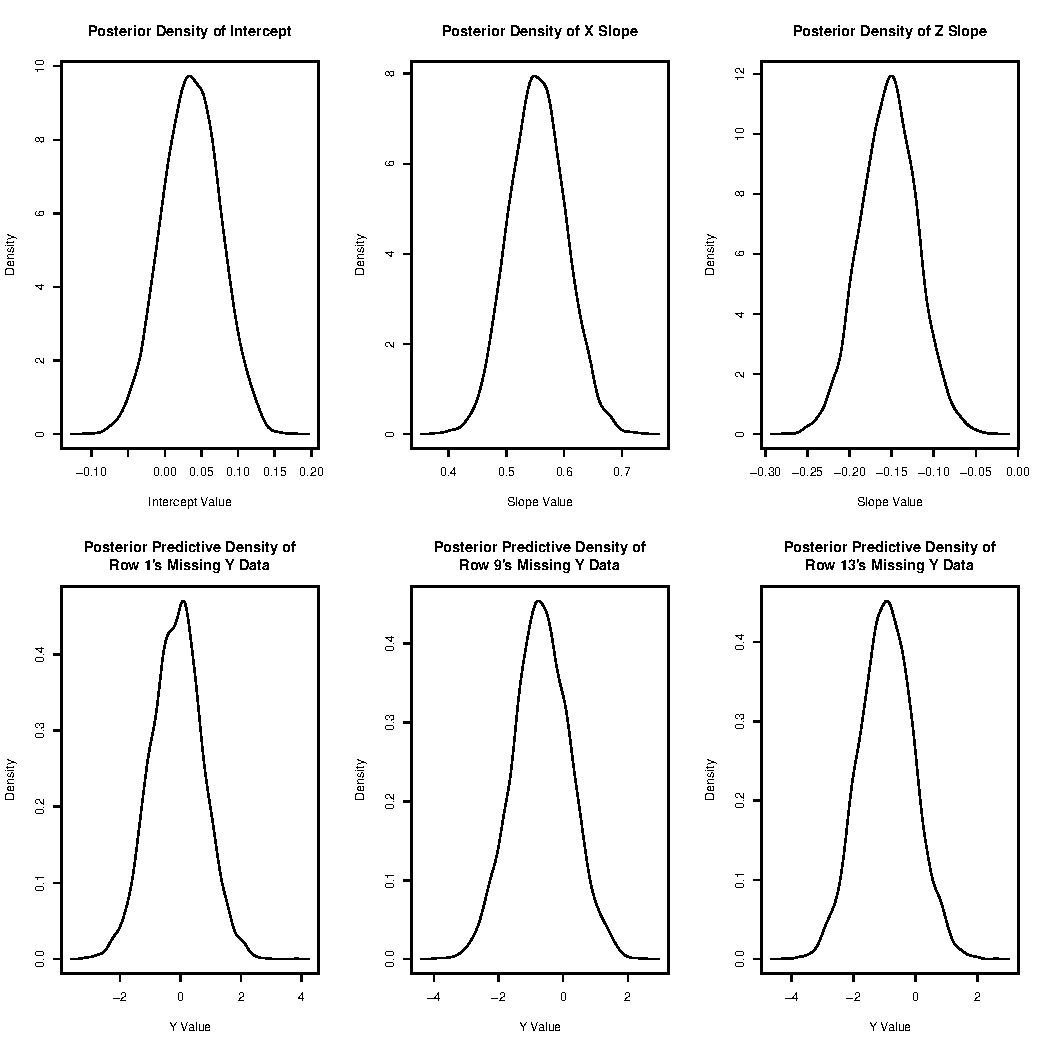
\includegraphics[width=0.65\linewidth]{figure/unnamed-chunk-15-1} 

}



\end{knitrout}

\end{frame}

\watermarkon %-----------------------------------------------------------------%

\begin{frame}{Doing MI-Based Analysis}
  
  An MI-based data analysis consists of three phases:
  \vb
  \begin{enumerate}
  \item The imputation phase \label{iStep}
    \begin{itemize}
    \item Replace missing values with $M$ plausible estimates.
    \item Produce $M$ completed datasets.
    \end{itemize}
    \vb
  \item The analysis phase \label{aStep}
    \begin{itemize}
    \item Estimate $M$ replicates of your analysis model.
    \item Fit the same model to each of the $M$ datasets from Step \ref{iStep}.
    \end{itemize}
    \vb
  \item The pooling phase
    \begin{itemize}
    \item Combine the $M$ sets of parameter estimates and standard errors from 
      Step \ref{aStep} into a single set of MI estimates.
    \item Use these pooled parameter estimates and standard errors for 
      inference.
    \end{itemize}
  \end{enumerate}
  
\end{frame}

%------------------------------------------------------------------------------%

\begin{frame}{Pooling MI Estimates}
  
  \citet{rubin:1987} formulated a simple set of pooling rules for MI estimates.
  \vb
  \begin{itemize}
  \item The MI point estimate of some interesting quantity, $Q^*$, is simply 
    the mean of the $M$ estimates, $\{\hat{Q}_m\}$:
    \begin{align*}
      Q^* &= \frac{1}{M} \sum_{m = 1}^M \hat{Q}_m\\
    \end{align*}
  \end{itemize}
  
\end{frame}

%------------------------------------------------------------------------------%

\begin{frame}{Pooling MI Estimates}
  
  The MI variability estimate, $T$, is a slightly more complex entity.
  \vb
  \begin{itemize}
  \item A weighted sum of the \emph{within-imputation} variance, $W$, and the 
    \emph{between-imputation} variance, $B$.
    \begin{align*}
      W &= \frac{1}{M} \sum_{m = 1}^M \widehat{SE}_{Q,m}^2\\
      B &= \frac{1}{M - 1} \sum_{m = 1}^M \left( \hat{Q}_m - Q^* \right)^2\\
      T &= W + \left( 1 + M^{-1} \right) B\\ 
      &= W + B + \frac{B}{M}
    \end{align*}
  \end{itemize}
  
\end{frame}

%------------------------------------------------------------------------------%

\begin{frame}{Inference with MI Estimates}
  
  After computing $Q^*$ and $T$, we combine them in the usual way to get test 
  statistics and confidence intervals.
  \begin{align*}
    t &= \frac{Q^* - Q_0}{\sqrt{T}}\\
    CI &= Q^* \pm t_{crit} \sqrt{T}
  \end{align*}
  
  We must take care with our \emph{df}, though.
  \begin{align*}
    df = (M - 1) \left[1 + \frac{W}{\left(1 + M^{-1}\right)B}\right]^2
  \end{align*}
  
\end{frame}

%------------------------------------------------------------------------------%

\begin{frame}{Fraction of Missing Information}
  
  In Lecture 4, we briefly discussed a very desirable measure of nonresponse: 
  \emph{fraction of missing information} (FMI).
  
  \begin{align*}
    FMI = \frac{r + \frac{2}{(df + 3)}}{r + 1} \approx \frac{(1 + M^{-1})B}{(1 + M^{-1})B + W} \rightarrow \frac{B}{B + W}
  \end{align*}
  where
  \begin{align*}
    r = \frac{(1 + M^{-1})B}{W}
  \end{align*}
  The FMI gives us a sense of how much the missing data (and their treatment) 
  have influence our parameter estimates.
  \vc
  \begin{itemize}
  \item We should report the FMI for an estimated parameter along with other 
    ancillary statistics (e.g., t-tests, p-values, effect sizes, etc.).
  \end{itemize}
  
\end{frame}

\watermarkoff %----------------------------------------------------------------%

\begin{frame}[fragile]{Example: Analysis \& Pooling}
  
  Analyze the multiply imputed datasets and pool results:
  
\begin{knitrout}\footnotesize
\definecolor{shadecolor}{rgb}{0.878, 0.918, 0.933}\color{fgcolor}\begin{kframe}
\begin{alltt}
\hlcom{## Use each dataset to estimate the analysis model:}
\hlstd{fits1} \hlkwb{<-} \hlkwd{lapply}\hlstd{(impList,}
                \hlkwa{function}\hlstd{(}\hlkwc{dat}\hlstd{)} \hlkwd{lm}\hlstd{(z} \hlopt{~} \hlstd{x} \hlopt{+} \hlstd{y,} \hlkwc{data} \hlstd{= dat)}
                \hlstd{)}

\hlcom{## Pool the results:}
\hlstd{pool1} \hlkwb{<-} \hlkwd{MIcombine}\hlstd{(fits1)}
\hlkwd{summary}\hlstd{(pool1,} \hlkwc{digits} \hlstd{=} \hlnum{3}\hlstd{)}
\end{alltt}
\begin{verbatim}
## Multiple imputation results:
##       MIcombine.default(fits1)
##               results     se  (lower  upper) missInfo
## (Intercept)  0.000765 0.0304 -0.0587  0.0603      3 %
## x            0.366918 0.0378  0.2928  0.4410     12 %
## y           -0.182703 0.0407 -0.2626 -0.1028     29 %
\end{verbatim}
\end{kframe}
\end{knitrout}

\end{frame}

\watermarkon %-----------------------------------------------------------------%

\begin{frame}[allowframebreaks]{Model-Based vs. Donor-Based Methods}
  
  They types of MI we've discussed above are all \emph{model-based}.
  \vc
  \begin{itemize}
  \item The imputations are randomly sampled from an estimated distribution of 
    the missing values (i.e., a probability \emph{model} of the missing data).
  \end{itemize}
  \vb
  Model-based methods are theoretically ideal when the missing data truly follow 
  the chosen distribution.
  \vc
  \begin{itemize}
  \item If the missing data do not follow the model, performance suffers.
  \end{itemize}
  \vb
  Sometimes, the solution is to employ a different probability model.
  \vc
  \begin{itemize}
  \item We'll see this approach when we discuss MI for categorical variables.
  \end{itemize}
  
  \pagebreak
  
  If we're not able to choose a sensible distribution for the missing data, we 
  can use \emph{Donor-Based Methods}.
  \vc
  \begin{itemize}
  \item Imputations are sampled from a pool of matched observed cases.
    \vc
  \item The empirical distribution of the observed data is preserved.
  \end{itemize}
  \vb
  One particularly useful donor-based method is \emph{Predictive Mean Matching} 
  \citep{little:1988}.
  \begin{itemize}
  \item The cases that make up the donor pool are matched based on their 
    predicted outcome values.
  \end{itemize}
  
\end{frame}

%------------------------------------------------------------------------------%

\begin{frame}[allowframebreaks]{Predictive Mean Matching: Procedure}
  
  Suppose we want to generate $M$ imputations for an incomplete variable, $Y$, 
  using some set of predictors, $\mathbf{X}$.
  \vc
  \begin{enumerate}
  \item Regress $Y_{obs}$ onto $\mathbf{X}_{obs}$ and compute the conditional mean 
    of $Y_{obs}$: 
    \begin{itemize}
    \item $\hat{\mu} = \mathbf{X}_{obs} \hat{\beta}$
    \end{itemize}
    \vc
  \item Do a Bayesian linear regression of $Y_{obs}$ onto $\mathbf{X}_{obs}$ and 
    sample $M$ values of the posterior predicted mean of $Y_{mis}$: 
    \begin{itemize}
    \item $\tilde{\mu}_m = \mathbf{X}_{mis} \tilde{\beta}_m$.
    \end{itemize}
    \vc
  \item Compute $M$ sets of the matching distances: 
    \begin{itemize}
    \item $d(i, j)_m = (\tilde{\mu}_{mi} - \hat{\mu}_j)^2,~~i = 1, 2, \ldots N_{mis},~~j = 1, 2, \ldots, N_{obs}.$
    \end{itemize}
    
    \pagebreak
    
  \item Use each $d(i, j)_m$ to construct $N_{mis}$ donor pools. \label{findPools}
    \begin{itemize} 
    \item Find the $K$ (e.g., $K \in \{3, 5, 10\}$) cases with the smallest 
      values of $d(1, j)_m$, $d(2, j)_m$, $\ldots$, $d(N_{mis}, j)_m$. 
    \end{itemize}
    \vc
  \item For $m = 1, 2, \ldots, M$, select the final donor cases by randomly 
    sampling a single observation from each of the $N_{mis}$ donor pools defined 
    in Step \ref{findPools}. \label{findDonors}
    \vc
  \item For each of the $M$ imputations replace the missing values in $Y$ with 
    the donor data selected in Step \ref{findDonors}.
  \end{enumerate}
  
\end{frame}

\watermarkoff %----------------------------------------------------------------%

\begin{frame}[fragile]{Predictive Mean Matching: Example}

  Compute/sample the appropriate conditional means:
  
\begin{knitrout}\footnotesize
\definecolor{shadecolor}{rgb}{0.878, 0.918, 0.933}\color{fgcolor}\begin{kframe}
\begin{alltt}
\hlcom{## Define donor pool size:}
\hlstd{K} \hlkwb{<-} \hlnum{5}

\hlcom{## Conditional mean of Y_mis:}
\hlstd{mu0} \hlkwb{<-} \hlkwd{predict}\hlstd{(fit0)}

\hlcom{## Posterior predicted means of Y_mis:}
\hlstd{mu1} \hlkwb{<-} \hlkwd{as.data.frame}\hlstd{(}
    \hlstd{misX} \hlopt \hlkwd{t}\hlstd{(betaSams[}\hlkwd{sample}\hlstd{(}\hlnum{1} \hlopt{:} \hlstd{nSams, nImps), ])}
\hlstd{)}
\end{alltt}
\end{kframe}
\end{knitrout}

\end{frame}

%------------------------------------------------------------------------------%

\begin{frame}[fragile]{Predictive Mean Matching: Example}

  Define a function to find donor cases:
  
\begin{knitrout}\footnotesize
\definecolor{shadecolor}{rgb}{0.878, 0.918, 0.933}\color{fgcolor}\begin{kframe}
\begin{alltt}
\hlstd{getDonors} \hlkwb{<-} \hlkwa{function}\hlstd{(}\hlkwc{x}\hlstd{,} \hlkwc{y}\hlstd{,} \hlkwc{K}\hlstd{) \{}
    \hlcom{## Compute distances:}
    \hlstd{d} \hlkwb{<-} \hlstd{(x} \hlopt{-} \hlstd{y)}\hlopt{^}\hlnum{2}

    \hlcom{## Indices of the K smallest distances:}
    \hlstd{ind} \hlkwb{<-} \hlkwd{which}\hlstd{(}\hlkwd{order}\hlstd{(d)} \hlopt \hlnum{1} \hlopt{:} \hlstd{K)}

    \hlcom{## Return a randomly sampled index:}
    \hlkwd{sample}\hlstd{(ind,} \hlnum{1}\hlstd{)}
\hlstd{\}}
\end{alltt}
\end{kframe}
\end{knitrout}

\end{frame}

%------------------------------------------------------------------------------%

\begin{frame}[fragile]{Predictive Mean Matching: Example}

  Implement the imputation:
  
\begin{knitrout}\footnotesize
\definecolor{shadecolor}{rgb}{0.878, 0.918, 0.933}\color{fgcolor}\begin{kframe}
\begin{alltt}
\hlstd{impList2} \hlkwb{<-} \hlkwd{list}\hlstd{()}
\hlkwa{for}\hlstd{(m} \hlkwa{in} \hlnum{1} \hlopt{:} \hlstd{nImps) \{}
    \hlcom{## Find donor cases:}
    \hlstd{d0} \hlkwb{<-} \hlkwd{sapply}\hlstd{(mu1[ , m], getDonors,} \hlkwc{y} \hlstd{= mu0,} \hlkwc{K} \hlstd{= K)}

    \hlcom{## Impute the missing values:}
    \hlstd{impData}            \hlkwb{<-} \hlstd{misData}
    \hlstd{impData[rVec,} \hlstr{"y"}\hlstd{]} \hlkwb{<-} \hlstd{yObs}\hlopt{$}\hlstd{y[d0]}

    \hlcom{## Save the imputed dataset:}
    \hlstd{impList2[[m]]} \hlkwb{<-} \hlstd{impData}
\hlstd{\}}
\end{alltt}
\end{kframe}
\end{knitrout}

\end{frame}

%------------------------------------------------------------------------------%

\begin{frame}[fragile]{Predictive Mean Matching: Example}
\begin{knitrout}\footnotesize
\definecolor{shadecolor}{rgb}{0.878, 0.918, 0.933}\color{fgcolor}\begin{kframe}
\begin{alltt}
\hlcom{## Use each dataset to estimate the analysis model:}
\hlstd{fits2} \hlkwb{<-} \hlkwd{lapply}\hlstd{(impList2,}
                \hlkwa{function}\hlstd{(}\hlkwc{dat}\hlstd{)} \hlkwd{lm}\hlstd{(z} \hlopt{~} \hlstd{x} \hlopt{+} \hlstd{y,} \hlkwc{data} \hlstd{= dat)}
                \hlstd{)}

\hlcom{## Pool the results:}
\hlstd{pool2} \hlkwb{<-} \hlkwd{MIcombine}\hlstd{(fits2)}
\hlkwd{summary}\hlstd{(pool2,} \hlkwc{digits} \hlstd{=} \hlnum{3}\hlstd{)}
\end{alltt}
\begin{verbatim}
## Multiple imputation results:
##       MIcombine.default(fits2)
##             results     se  (lower  upper) missInfo
## (Intercept)  0.0277 0.0323 -0.0357  0.0910      4 %
## x            0.2805 0.0313  0.2191  0.3419      1 %
## y           -0.0940 0.0330 -0.1589 -0.0292     32 %
\end{verbatim}
\end{kframe}
\end{knitrout}

\end{frame}

\watermarkon %-----------------------------------------------------------------%

\begin{frame}{Pros and Cons of Predictive Mean Matching}
  
  PMM tends to work well with continuous, non-normal variables.
  \begin{itemize}
  \item Relatively robust to misspecification of the imputation model
  \item Imputed values are always valid
  \end{itemize}
  \vb
  PMM does have some important limitations.
  \begin{itemize}
  \item In small samples, the same donor cases can be re-used many times.
  \item PMM cannot extrapolate beyond the observed range of the data.
  \item PMM cannot be used with some variable types.
    \begin{itemize}
    \item Nominal variables
    \end{itemize}
  \item PMM may perform poorly when the number of predictor variables is small.
  \end{itemize}
  
\end{frame}

%------------------------------------------------------------------------------%

\begin{frame}[allowframebreaks]{References}
  
  \bibliographystyle{apacite}
  \bibliography{../../../literature/bibtexFiles/statMethRefs.bib,../../../literature/bibtexFiles/dissRefsList.bib}
  
\end{frame}

%------------------------------------------------------------------------------%

\end{document}

